\documentclass[]{article}
\usepackage{lmodern}
\usepackage{amssymb,amsmath}
\usepackage{ifxetex,ifluatex}
\usepackage{fixltx2e} % provides \textsubscript
\ifnum 0\ifxetex 1\fi\ifluatex 1\fi=0 % if pdftex
  \usepackage[T1]{fontenc}
  \usepackage[utf8]{inputenc}
\else % if luatex or xelatex
  \ifxetex
    \usepackage{mathspec}
  \else
    \usepackage{fontspec}
  \fi
  \defaultfontfeatures{Ligatures=TeX,Scale=MatchLowercase}
\fi
% use upquote if available, for straight quotes in verbatim environments
\IfFileExists{upquote.sty}{\usepackage{upquote}}{}
% use microtype if available
\IfFileExists{microtype.sty}{%
\usepackage{microtype}
\UseMicrotypeSet[protrusion]{basicmath} % disable protrusion for tt fonts
}{}
\usepackage[margin=1in]{geometry}
\usepackage{hyperref}
\hypersetup{unicode=true,
            pdftitle={Liver Disease Classification},
            pdfauthor={Nabeel Khan},
            pdfborder={0 0 0},
            breaklinks=true}
\urlstyle{same}  % don't use monospace font for urls
\usepackage{color}
\usepackage{fancyvrb}
\newcommand{\VerbBar}{|}
\newcommand{\VERB}{\Verb[commandchars=\\\{\}]}
\DefineVerbatimEnvironment{Highlighting}{Verbatim}{commandchars=\\\{\}}
% Add ',fontsize=\small' for more characters per line
\usepackage{framed}
\definecolor{shadecolor}{RGB}{248,248,248}
\newenvironment{Shaded}{\begin{snugshade}}{\end{snugshade}}
\newcommand{\AlertTok}[1]{\textcolor[rgb]{0.94,0.16,0.16}{#1}}
\newcommand{\AnnotationTok}[1]{\textcolor[rgb]{0.56,0.35,0.01}{\textbf{\textit{#1}}}}
\newcommand{\AttributeTok}[1]{\textcolor[rgb]{0.77,0.63,0.00}{#1}}
\newcommand{\BaseNTok}[1]{\textcolor[rgb]{0.00,0.00,0.81}{#1}}
\newcommand{\BuiltInTok}[1]{#1}
\newcommand{\CharTok}[1]{\textcolor[rgb]{0.31,0.60,0.02}{#1}}
\newcommand{\CommentTok}[1]{\textcolor[rgb]{0.56,0.35,0.01}{\textit{#1}}}
\newcommand{\CommentVarTok}[1]{\textcolor[rgb]{0.56,0.35,0.01}{\textbf{\textit{#1}}}}
\newcommand{\ConstantTok}[1]{\textcolor[rgb]{0.00,0.00,0.00}{#1}}
\newcommand{\ControlFlowTok}[1]{\textcolor[rgb]{0.13,0.29,0.53}{\textbf{#1}}}
\newcommand{\DataTypeTok}[1]{\textcolor[rgb]{0.13,0.29,0.53}{#1}}
\newcommand{\DecValTok}[1]{\textcolor[rgb]{0.00,0.00,0.81}{#1}}
\newcommand{\DocumentationTok}[1]{\textcolor[rgb]{0.56,0.35,0.01}{\textbf{\textit{#1}}}}
\newcommand{\ErrorTok}[1]{\textcolor[rgb]{0.64,0.00,0.00}{\textbf{#1}}}
\newcommand{\ExtensionTok}[1]{#1}
\newcommand{\FloatTok}[1]{\textcolor[rgb]{0.00,0.00,0.81}{#1}}
\newcommand{\FunctionTok}[1]{\textcolor[rgb]{0.00,0.00,0.00}{#1}}
\newcommand{\ImportTok}[1]{#1}
\newcommand{\InformationTok}[1]{\textcolor[rgb]{0.56,0.35,0.01}{\textbf{\textit{#1}}}}
\newcommand{\KeywordTok}[1]{\textcolor[rgb]{0.13,0.29,0.53}{\textbf{#1}}}
\newcommand{\NormalTok}[1]{#1}
\newcommand{\OperatorTok}[1]{\textcolor[rgb]{0.81,0.36,0.00}{\textbf{#1}}}
\newcommand{\OtherTok}[1]{\textcolor[rgb]{0.56,0.35,0.01}{#1}}
\newcommand{\PreprocessorTok}[1]{\textcolor[rgb]{0.56,0.35,0.01}{\textit{#1}}}
\newcommand{\RegionMarkerTok}[1]{#1}
\newcommand{\SpecialCharTok}[1]{\textcolor[rgb]{0.00,0.00,0.00}{#1}}
\newcommand{\SpecialStringTok}[1]{\textcolor[rgb]{0.31,0.60,0.02}{#1}}
\newcommand{\StringTok}[1]{\textcolor[rgb]{0.31,0.60,0.02}{#1}}
\newcommand{\VariableTok}[1]{\textcolor[rgb]{0.00,0.00,0.00}{#1}}
\newcommand{\VerbatimStringTok}[1]{\textcolor[rgb]{0.31,0.60,0.02}{#1}}
\newcommand{\WarningTok}[1]{\textcolor[rgb]{0.56,0.35,0.01}{\textbf{\textit{#1}}}}
\usepackage{longtable,booktabs}
\usepackage{graphicx,grffile}
\makeatletter
\def\maxwidth{\ifdim\Gin@nat@width>\linewidth\linewidth\else\Gin@nat@width\fi}
\def\maxheight{\ifdim\Gin@nat@height>\textheight\textheight\else\Gin@nat@height\fi}
\makeatother
% Scale images if necessary, so that they will not overflow the page
% margins by default, and it is still possible to overwrite the defaults
% using explicit options in \includegraphics[width, height, ...]{}
\setkeys{Gin}{width=\maxwidth,height=\maxheight,keepaspectratio}
\IfFileExists{parskip.sty}{%
\usepackage{parskip}
}{% else
\setlength{\parindent}{0pt}
\setlength{\parskip}{6pt plus 2pt minus 1pt}
}
\setlength{\emergencystretch}{3em}  % prevent overfull lines
\providecommand{\tightlist}{%
  \setlength{\itemsep}{0pt}\setlength{\parskip}{0pt}}
\setcounter{secnumdepth}{5}
% Redefines (sub)paragraphs to behave more like sections
\ifx\paragraph\undefined\else
\let\oldparagraph\paragraph
\renewcommand{\paragraph}[1]{\oldparagraph{#1}\mbox{}}
\fi
\ifx\subparagraph\undefined\else
\let\oldsubparagraph\subparagraph
\renewcommand{\subparagraph}[1]{\oldsubparagraph{#1}\mbox{}}
\fi

%%% Use protect on footnotes to avoid problems with footnotes in titles
\let\rmarkdownfootnote\footnote%
\def\footnote{\protect\rmarkdownfootnote}

%%% Change title format to be more compact
\usepackage{titling}

% Create subtitle command for use in maketitle
\providecommand{\subtitle}[1]{
  \posttitle{
    \begin{center}\large#1\end{center}
    }
}

\setlength{\droptitle}{-2em}

  \title{Liver Disease Classification}
    \pretitle{\vspace{\droptitle}\centering\huge}
  \posttitle{\par}
    \author{Nabeel Khan}
    \preauthor{\centering\large\emph}
  \postauthor{\par}
      \predate{\centering\large\emph}
  \postdate{\par}
    \date{27-May-2020}


\begin{document}
\maketitle

{
\setcounter{tocdepth}{2}
\tableofcontents
}
\section{Introduction}
\label{sec:introduction}

This report is part of the `HarvardX: PH125.9x Data Science: Capstone'
course. In this report, we chose a dataset of our choice and apply
various machine learning techniques to perform binary classification to
diagnose liver disease.

\subsection{Background}
\label{sec:background}

The liver plays an important role in keeping us healthy. The main job of
liver is to filter the blood coming from the digestive tract, before
passing it to the rest of the body. The liver also turns nutrients into
chemicals our body needs, turns food into energy, and filters out
poisons. So, malfunctioing of liver affects the whole body.

The classification techniques are used in various automatic medical
diagnoses tools\cite{cad}.The problems with liver patients are not
easily discovered in an early stage. An early diagnosis of liver
problems will help in increasing the survival rate of patiets. We can
detect the liver disease by analyzing the levels of enzymes in the blood
\cite{ld,bendi}. A classification algorithm capable of automatically
detecting the liver disease can assisst the doctors.

\subsection{Aim of Project}
\label{sec:aim}

The patients with liver disease are on the rise because of excessive
consumption of alcohol, inhale of harmful gases, intake of contaminated
food, pickles and drugs. The aim of this proect is to develop a bianry
classifier, which can use blood enzymes information to diagnose liver
disease.

\section{Dataset and Evaluation Metrics}
\label{sec:dataset}

We use the Liver Patient Records, which are collected from North East of
Andhra Pradesh, India. The data set contains:

\begin{enumerate}
\item 416 liver patient records and 167 non-liver patient records.
\end{enumerate}

\subsection{Download Data}
\label{sec:dd}

The dataset is publically available online both at Kaggle and UCI
repository. We download data from the website. Then, we split data into
a training and validation sets.

\begin{itemize}
\item 10\% of the data is used for validation, and 90% is used for training.
\end{itemize}

\begin{Shaded}
\begin{Highlighting}[]
\CommentTok{################################}
\CommentTok{#  Install packages (if not installed)}
\CommentTok{################################}
\CommentTok{# Note: this process could take a couple of minutes}
\NormalTok{repos_path<-}\StringTok{ "http://cran.us.r-project.org"}
\ControlFlowTok{if}\NormalTok{(}\OperatorTok{!}\KeywordTok{require}\NormalTok{(tidyverse)) }\KeywordTok{install.packages}\NormalTok{(}\StringTok{"tidyverse"}\NormalTok{, }\DataTypeTok{repos =}\NormalTok{repos_path)}
\end{Highlighting}
\end{Shaded}

\begin{verbatim}
## Loading required package: tidyverse
\end{verbatim}

\begin{verbatim}
## -- Attaching packages --------------------------------------------------- tidyverse 1.3.0 --
\end{verbatim}

\begin{verbatim}
## v ggplot2 3.2.1     v purrr   0.3.3
## v tibble  2.1.3     v dplyr   0.8.3
## v tidyr   1.0.0     v stringr 1.4.0
## v readr   1.3.1     v forcats 0.4.0
\end{verbatim}

\begin{verbatim}
## -- Conflicts ------------------------------------------------------ tidyverse_conflicts() --
## x dplyr::filter() masks stats::filter()
## x dplyr::lag()    masks stats::lag()
\end{verbatim}

\begin{Shaded}
\begin{Highlighting}[]
\ControlFlowTok{if}\NormalTok{(}\OperatorTok{!}\KeywordTok{require}\NormalTok{(caret)) }\KeywordTok{install.packages}\NormalTok{(}\StringTok{"caret"}\NormalTok{, }\DataTypeTok{repos =}\NormalTok{ repos_path)}
\end{Highlighting}
\end{Shaded}

\begin{verbatim}
## Loading required package: caret
\end{verbatim}

\begin{verbatim}
## Loading required package: lattice
\end{verbatim}

\begin{verbatim}
## 
## Attaching package: 'caret'
\end{verbatim}

\begin{verbatim}
## The following object is masked from 'package:purrr':
## 
##     lift
\end{verbatim}

\begin{Shaded}
\begin{Highlighting}[]
\ControlFlowTok{if}\NormalTok{(}\OperatorTok{!}\KeywordTok{require}\NormalTok{(data.table)) }\KeywordTok{install.packages}\NormalTok{(}\StringTok{"data.table"}\NormalTok{, }\DataTypeTok{repos =}\NormalTok{repos_path)}
\end{Highlighting}
\end{Shaded}

\begin{verbatim}
## Loading required package: data.table
\end{verbatim}

\begin{verbatim}
## 
## Attaching package: 'data.table'
\end{verbatim}

\begin{verbatim}
## The following objects are masked from 'package:dplyr':
## 
##     between, first, last
\end{verbatim}

\begin{verbatim}
## The following object is masked from 'package:purrr':
## 
##     transpose
\end{verbatim}

\begin{Shaded}
\begin{Highlighting}[]
\ControlFlowTok{if}\NormalTok{(}\OperatorTok{!}\KeywordTok{require}\NormalTok{(lubridate)) }\KeywordTok{install.packages}\NormalTok{(}\StringTok{"lubridate"}\NormalTok{, }\DataTypeTok{repos =}\NormalTok{ repos_path)}
\end{Highlighting}
\end{Shaded}

\begin{verbatim}
## Loading required package: lubridate
\end{verbatim}

\begin{verbatim}
## 
## Attaching package: 'lubridate'
\end{verbatim}

\begin{verbatim}
## The following objects are masked from 'package:data.table':
## 
##     hour, isoweek, mday, minute, month, quarter, second, wday,
##     week, yday, year
\end{verbatim}

\begin{verbatim}
## The following object is masked from 'package:base':
## 
##     date
\end{verbatim}

\begin{Shaded}
\begin{Highlighting}[]
\ControlFlowTok{if}\NormalTok{(}\OperatorTok{!}\KeywordTok{require}\NormalTok{(dplyr)) }\KeywordTok{install.packages}\NormalTok{(}\StringTok{"dplyr"}\NormalTok{, }\DataTypeTok{repos =}\NormalTok{ repos_path)}
\ControlFlowTok{if}\NormalTok{(}\OperatorTok{!}\KeywordTok{require}\NormalTok{(sjmisc)) }\KeywordTok{install.packages}\NormalTok{(}\StringTok{"dplyr"}\NormalTok{, }\DataTypeTok{repos =}\NormalTok{ repos_path)}
\end{Highlighting}
\end{Shaded}

\begin{verbatim}
## Loading required package: sjmisc
\end{verbatim}

\begin{verbatim}
## 
## Attaching package: 'sjmisc'
\end{verbatim}

\begin{verbatim}
## The following object is masked from 'package:purrr':
## 
##     is_empty
\end{verbatim}

\begin{verbatim}
## The following object is masked from 'package:tidyr':
## 
##     replace_na
\end{verbatim}

\begin{verbatim}
## The following object is masked from 'package:tibble':
## 
##     add_case
\end{verbatim}

\begin{Shaded}
\begin{Highlighting}[]
\ControlFlowTok{if}\NormalTok{(}\OperatorTok{!}\KeywordTok{require}\NormalTok{(sjmisc)) }\KeywordTok{install.packages}\NormalTok{(}\StringTok{"scales"}\NormalTok{, }\DataTypeTok{repos =}\NormalTok{ repos_path)}

\CommentTok{################################}
\CommentTok{# Load libraries}
\CommentTok{################################}
\KeywordTok{library}\NormalTok{(lubridate)}
\KeywordTok{library}\NormalTok{(tidyverse)}
\KeywordTok{library}\NormalTok{(dplyr)}
\KeywordTok{library}\NormalTok{(lubridate)}
\KeywordTok{library}\NormalTok{(sjmisc)}
\KeywordTok{library}\NormalTok{(scales)}
\end{Highlighting}
\end{Shaded}

\begin{verbatim}
## 
## Attaching package: 'scales'
\end{verbatim}

\begin{verbatim}
## The following object is masked from 'package:purrr':
## 
##     discard
\end{verbatim}

\begin{verbatim}
## The following object is masked from 'package:readr':
## 
##     col_factor
\end{verbatim}

\begin{Shaded}
\begin{Highlighting}[]
\CommentTok{################################}
\CommentTok{# Downloading data}
\CommentTok{################################}
\CommentTok{# Indian Live Patient Records :}
 \CommentTok{# https://www.kaggle.com/uciml/indian-liver-patient-records/}
 \CommentTok{# https://archive.ics.uci.edu/ml/machine-learning-databases/00225/Indian Liver Patient Dataset (ILPD).csv}

\NormalTok{url <-}\StringTok{ "https://archive.ics.uci.edu/ml/machine-learning-databases/00225/Indian Liver Patient Dataset (ILPD).csv"}
\CommentTok{# Download csv}
\NormalTok{liverData <-}\StringTok{ }\KeywordTok{read.csv}\NormalTok{(url)}

\CommentTok{# Rename columns of csv}
\KeywordTok{colnames}\NormalTok{(liverData)<-}\StringTok{ }\KeywordTok{c}\NormalTok{(}\StringTok{"Age"}\NormalTok{,}\StringTok{"Gender"}\NormalTok{,}\StringTok{"Total_Bilirubin"}\NormalTok{,}\StringTok{"Direct_Bilirubin"}\NormalTok{, }\StringTok{"Alkaline_Phosphotase"}\NormalTok{,}\StringTok{"Alamine_Aminotransferase"}\NormalTok{,}\StringTok{"Aspartate_Aminotransferase"}\NormalTok{,    }\StringTok{"Total_Protiens"}\NormalTok{,}\StringTok{"Albumin"}\NormalTok{,}\StringTok{"Albumin_and_Globulin_Ratio"}\NormalTok{,}\StringTok{"Dataset"}\NormalTok{)}

\CommentTok{################################}
\CommentTok{# Creating training and validation sets}
\CommentTok{################################}

\CommentTok{# Validation set will be 10% of whole data}
\KeywordTok{set.seed}\NormalTok{(}\DecValTok{1}\NormalTok{, }\DataTypeTok{sample.kind =} \StringTok{"Rounding"}\NormalTok{)}
\end{Highlighting}
\end{Shaded}

\begin{verbatim}
## Warning in set.seed(1, sample.kind = "Rounding"): non-uniform 'Rounding'
## sampler used
\end{verbatim}

\begin{Shaded}
\begin{Highlighting}[]
\NormalTok{test_index <-}\StringTok{ }\KeywordTok{createDataPartition}\NormalTok{(}\DataTypeTok{y =}\NormalTok{ liverData}\OperatorTok{$}\NormalTok{Dataset, }\DataTypeTok{times =} \DecValTok{1}\NormalTok{, }\DataTypeTok{p =} \FloatTok{0.1}\NormalTok{, }\DataTypeTok{list =} \OtherTok{FALSE}\NormalTok{)}

\NormalTok{training <-}\StringTok{ }\NormalTok{liverData[}\OperatorTok{-}\NormalTok{test_index,]}
\NormalTok{validation <-}\StringTok{ }\NormalTok{liverData[test_index,]}

 \CommentTok{# Removing the objects from environment as no longer required}
\KeywordTok{rm}\NormalTok{(liverData)}
\end{Highlighting}
\end{Shaded}

\subsection{Metrics}
\label{sec:metrics}

To evaluate the performance of classifiers, we will use following
metrics:

\begin{enumerate}
\item \textbf{Accuracy}
It is the ratio of number of correct predictions to the total number of input samples.
\begin{equation}
Accuracy = \frac{True positives + True negatives} {Total Predictions}
\end{equation}

\item \textbf{Sensitivity}
It is also referred as true positive rate or recall. It is the proportion of true positives that are correctly identified.

\begin{equation}
Sensitivity = \frac{Number of true positives} {Number of true positives + Number of false negatives}
\end{equation}

\item \textbf{Precision}
It is defined as the proportion of the true positives against all the positive
results.

\begin{equation}
Precision = \frac{Number of true positives} {Number of true positives + Number of false positives}
\end{equation}

\item \textbf{Specificity}
It is the True negative rate. It is the proportion of true negatives that are
correctly identified.

\begin{equation}
Specificity = \frac{Number of true negatives} {Number of true negatives + Number of false positives}
\end{equation}

\item \textbf{F1 Score}
One metric that is preferred over overall accuracy is the average of specificity and sensitivity, referred to as balanced accuracy. Because specificity and sensitivity are rates, it is more appropriate to compute the harmonic average. In fact, the F1-score is widely used to compute harmonic average of precision and recall.

\begin{equation}
F1 Score = 2 * \frac{Precision - Recall} {Precision + Recall}
\end{equation}

\end{enumerate}

\section{Data Exploration}
\label{sec:exploration}

The dataset contains 11 variables namely,
`Age',`Gender',`Total\_Bilirubin', or ``Alkaline\_Phosphotase''. The
`Dataset' variable indicates if the liver has a disease or not. For
instance, a value of 1 indicates a disease and 2 indicates no disease.

All other variables except \texttt{Age",}Gender``, and ``Dataset''
represent the amount of enzymes in the blood. These variables will be
used to train our machine learning models for making predictions or
diagnosis.

\small

\begin{Shaded}
\begin{Highlighting}[]
\KeywordTok{head}\NormalTok{(training)}
\end{Highlighting}
\end{Shaded}

\begin{longtable}[]{@{}rlrrrrrrrrr@{}}
\toprule
Age & Gender & Total\_Bilirubin & Direct\_Bilirubin &
Alkaline\_Phosphotase & Alamine\_Aminotransferase &
Aspartate\_Aminotransferase & Total\_Protiens & Albumin &
Albumin\_and\_Globulin\_Ratio & Dataset\tabularnewline
\midrule
\endhead
62 & Male & 10.9 & 5.5 & 699 & 64 & 100 & 7.5 & 3.2 & 0.74 &
1\tabularnewline
62 & Male & 7.3 & 4.1 & 490 & 60 & 68 & 7.0 & 3.3 & 0.89 &
1\tabularnewline
58 & Male & 1.0 & 0.4 & 182 & 14 & 20 & 6.8 & 3.4 & 1.00 &
1\tabularnewline
72 & Male & 3.9 & 2.0 & 195 & 27 & 59 & 7.3 & 2.4 & 0.40 &
1\tabularnewline
46 & Male & 1.8 & 0.7 & 208 & 19 & 14 & 7.6 & 4.4 & 1.30 &
1\tabularnewline
26 & Female & 0.9 & 0.2 & 154 & 16 & 12 & 7.0 & 3.5 & 1.00 &
1\tabularnewline
\bottomrule
\end{longtable}

The training dataset has 523 records and there are no null values
(confirmed using summary).

\begin{Shaded}
\begin{Highlighting}[]
\KeywordTok{sprintf}\NormalTok{(}\StringTok{"Rows of training dataset = %d"}\NormalTok{, }\KeywordTok{nrow}\NormalTok{(training))}
\end{Highlighting}
\end{Shaded}

\begin{verbatim}
## [1] "Rows of training dataset = 523"
\end{verbatim}

\begin{Shaded}
\begin{Highlighting}[]
\KeywordTok{print}\NormalTok{(}\StringTok{"========================="}\NormalTok{)}
\end{Highlighting}
\end{Shaded}

\begin{verbatim}
## [1] "========================="
\end{verbatim}

\begin{Shaded}
\begin{Highlighting}[]
\KeywordTok{summary}\NormalTok{(training)}
\end{Highlighting}
\end{Shaded}

\begin{verbatim}
##       Age           Gender    Total_Bilirubin Direct_Bilirubin
##  Min.   : 4.00   Female:125   Min.   : 0.40   Min.   : 0.100  
##  1st Qu.:33.00   Male  :398   1st Qu.: 0.80   1st Qu.: 0.200  
##  Median :45.00                Median : 1.00   Median : 0.300  
##  Mean   :45.33                Mean   : 3.22   Mean   : 1.446  
##  3rd Qu.:58.00                3rd Qu.: 2.60   3rd Qu.: 1.300  
##  Max.   :90.00                Max.   :75.00   Max.   :19.700  
##                                                               
##  Alkaline_Phosphotase Alamine_Aminotransferase Aspartate_Aminotransferase
##  Min.   :  63.0       Min.   :  10.00          Min.   :  10.0            
##  1st Qu.: 176.0       1st Qu.:  24.00          1st Qu.:  25.0            
##  Median : 208.0       Median :  35.00          Median :  41.0            
##  Mean   : 289.9       Mean   :  76.34          Mean   : 105.0            
##  3rd Qu.: 298.0       3rd Qu.:  60.00          3rd Qu.:  86.5            
##  Max.   :1896.0       Max.   :1680.00          Max.   :4929.0            
##                                                                          
##  Total_Protiens    Albumin      Albumin_and_Globulin_Ratio    Dataset     
##  Min.   :2.70   Min.   :0.900   Min.   :0.3000             Min.   :1.000  
##  1st Qu.:5.80   1st Qu.:2.600   1st Qu.:0.7000             1st Qu.:1.000  
##  Median :6.60   Median :3.100   Median :0.9300             Median :1.000  
##  Mean   :6.49   Mean   :3.147   Mean   :0.9458             Mean   :1.281  
##  3rd Qu.:7.20   3rd Qu.:3.800   3rd Qu.:1.1000             3rd Qu.:2.000  
##  Max.   :9.50   Max.   :5.500   Max.   :2.8000             Max.   :2.000  
##                                 NA's   :4
\end{verbatim}

\subsubsection{Data Wrangling}
\label{sec:dw}

The variable ``Dataset" is our prediction and we will use it to analyse
the performance of machine lerning models. To improve readability, we
create a new column namely ``Liver Disease'', which will have two
values:

\begin{enumerate}
\item Malignant (M) indicating that the patienit has a liver disease.
\item Benign (B) indicating that the patient has no no liver disease.
\end{enumerate}

After creating a new column, wr delete the `Dataset' variable. We apply
these operations to both training and validation datasets.

\begin{Shaded}
\begin{Highlighting}[]
\CommentTok{# Adding a new column, which will contain the disease information}
\NormalTok{training <-}\StringTok{ }\KeywordTok{transform}\NormalTok{(training, }\DataTypeTok{Disease=} \KeywordTok{ifelse}\NormalTok{(Dataset}\OperatorTok{==}\DecValTok{1}\NormalTok{, }\StringTok{"M"}\NormalTok{,}\StringTok{"B"}\NormalTok{))}
\NormalTok{validation <-}\StringTok{ }\KeywordTok{transform}\NormalTok{(validation, }\DataTypeTok{Disease=} \KeywordTok{ifelse}\NormalTok{(Dataset}\OperatorTok{==}\DecValTok{1}\NormalTok{, }\StringTok{"M"}\NormalTok{,}\StringTok{"B"}\NormalTok{))}

\CommentTok{# Deleting the column 'Dataset' as no longer required}
\NormalTok{training<-}\KeywordTok{within}\NormalTok{(training, }\KeywordTok{rm}\NormalTok{(Dataset))}
\NormalTok{validation<-}\KeywordTok{within}\NormalTok{(validation, }\KeywordTok{rm}\NormalTok{(Dataset))}

\CommentTok{# Displaying the first siz rows}
\KeywordTok{head}\NormalTok{(training)}
\end{Highlighting}
\end{Shaded}

\begin{longtable}[]{@{}rlrrrrrrrrl@{}}
\toprule
Age & Gender & Total\_Bilirubin & Direct\_Bilirubin &
Alkaline\_Phosphotase & Alamine\_Aminotransferase &
Aspartate\_Aminotransferase & Total\_Protiens & Albumin &
Albumin\_and\_Globulin\_Ratio & Disease\tabularnewline
\midrule
\endhead
62 & Male & 10.9 & 5.5 & 699 & 64 & 100 & 7.5 & 3.2 & 0.74 &
M\tabularnewline
62 & Male & 7.3 & 4.1 & 490 & 60 & 68 & 7.0 & 3.3 & 0.89 &
M\tabularnewline
58 & Male & 1.0 & 0.4 & 182 & 14 & 20 & 6.8 & 3.4 & 1.00 &
M\tabularnewline
72 & Male & 3.9 & 2.0 & 195 & 27 & 59 & 7.3 & 2.4 & 0.40 &
M\tabularnewline
46 & Male & 1.8 & 0.7 & 208 & 19 & 14 & 7.6 & 4.4 & 1.30 &
M\tabularnewline
26 & Female & 0.9 & 0.2 & 154 & 16 & 12 & 7.0 & 3.5 & 1.00 &
M\tabularnewline
\bottomrule
\end{longtable}

\section{Data Analysis}
\label{sec:dataanalysis}

In this section, we extract insights from all variables to get in depth
understanding.

\subsection{Age}

The dataset consists of patients with varying ages, which makes this
dataset robust and un-biased towards a specific age group.

\begin{Shaded}
\begin{Highlighting}[]
\CommentTok{# Extracting frequency of patient ages}
\NormalTok{age_stats <-}\KeywordTok{as.data.frame}\NormalTok{(}\KeywordTok{table}\NormalTok{(training}\OperatorTok{$}\NormalTok{Age))}
\KeywordTok{names}\NormalTok{(age_stats)<-}\StringTok{ }\KeywordTok{c}\NormalTok{(}\StringTok{"Age"}\NormalTok{,}\StringTok{"Count"}\NormalTok{)}
\CommentTok{# Remvoing the factor}
\NormalTok{age_stats}\OperatorTok{$}\NormalTok{Age<-}\KeywordTok{as.numeric}\NormalTok{(}\KeywordTok{levels}\NormalTok{(age_stats}\OperatorTok{$}\NormalTok{Age))}

\CommentTok{# Plotting distribution of ages}
\NormalTok{age_stats }\OperatorTok\StringTok{ }\KeywordTok{ggplot}\NormalTok{(}\KeywordTok{aes}\NormalTok{(Age, Count)) }\OperatorTok{+}
\StringTok{  }\KeywordTok{geom_point}\NormalTok{(}\DataTypeTok{color=}\StringTok{"cadetblue"}\NormalTok{) }\OperatorTok{+}
\StringTok{  }\KeywordTok{scale_x_continuous}\NormalTok{(}\DataTypeTok{breaks =} \KeywordTok{round}\NormalTok{(}\KeywordTok{seq}\NormalTok{(}\KeywordTok{min}\NormalTok{(age_stats}\OperatorTok{$}\NormalTok{Age), }\KeywordTok{max}\NormalTok{(age_stats}\OperatorTok{$}\NormalTok{Age), }\DataTypeTok{by =} \DecValTok{6}\NormalTok{),}\DecValTok{1}\NormalTok{)) }\OperatorTok{+}
\StringTok{  }\KeywordTok{ggtitle}\NormalTok{(}\StringTok{"Distribution of Patient Ages"}\NormalTok{)}
\end{Highlighting}
\end{Shaded}

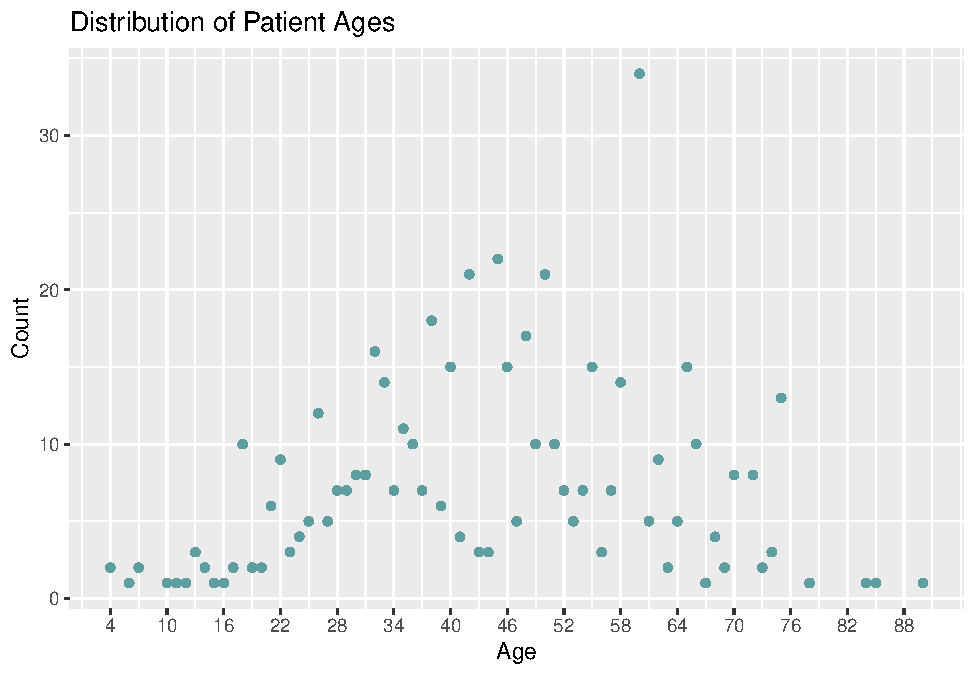
\includegraphics{LiverDisease_files/figure-latex/unnamed-chunk-6-1.pdf}
We analyse the age distributions with respect to the liver disease. The
distributions again suggest a good spread of age group.

\begin{Shaded}
\begin{Highlighting}[]
\CommentTok{# Plotting distributions of ages versus liver diseases}
\NormalTok{training }\OperatorTok\StringTok{ }
\StringTok{  }\KeywordTok{ggplot}\NormalTok{(}\KeywordTok{aes}\NormalTok{(}\KeywordTok{as.numeric}\NormalTok{(}\KeywordTok{row.names}\NormalTok{(training)),Age, }\DataTypeTok{color=}\NormalTok{Disease)) }\OperatorTok{+}
\StringTok{  }\KeywordTok{geom_point}\NormalTok{() }\OperatorTok{+}
\StringTok{  }\KeywordTok{labs}\NormalTok{(}\DataTypeTok{y=}\StringTok{"Age"}\NormalTok{, }\DataTypeTok{x =} \StringTok{"Number of patients"}\NormalTok{)}\OperatorTok{+}
\StringTok{  }\KeywordTok{facet_wrap}\NormalTok{( }\OperatorTok{~}\StringTok{ }\NormalTok{Disease) }\OperatorTok{+}
\StringTok{  }\KeywordTok{ggtitle}\NormalTok{(}\StringTok{"Distribution of ages w.r.t liver disease"}\NormalTok{)}
\end{Highlighting}
\end{Shaded}

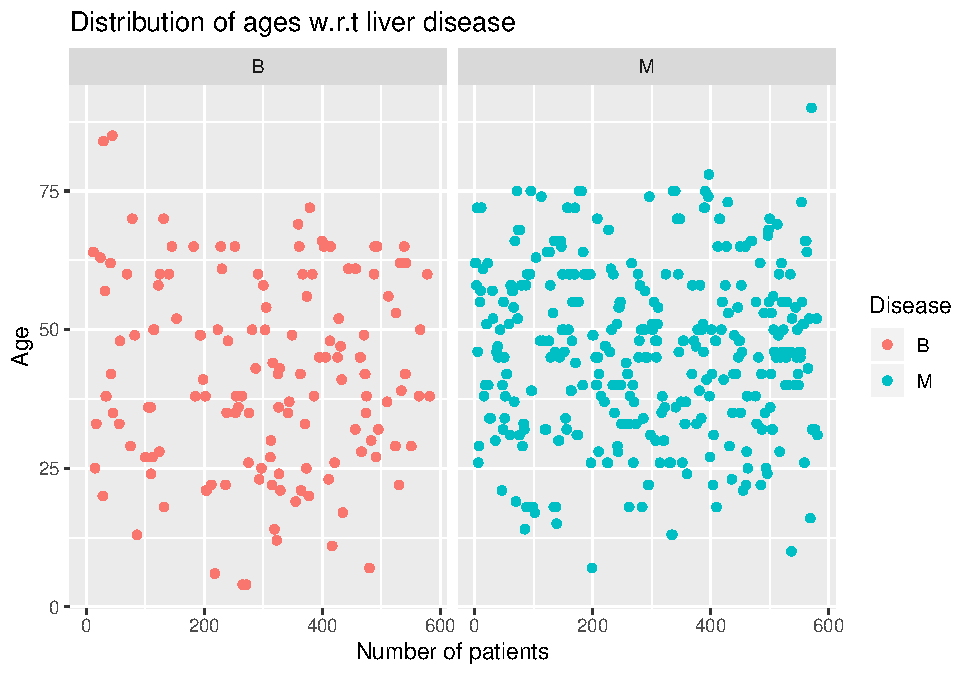
\includegraphics{LiverDisease_files/figure-latex/unnamed-chunk-7-1.pdf}

\subsection{Gender}

The analysis indicates that 76\% of the patient records belong to males.
It would have been good to have more and less equal distribution of
genders. Although, it may not make difference in the performance of
models.

\begin{Shaded}
\begin{Highlighting}[]
\CommentTok{# Getting summary of genders}
\KeywordTok{summary}\NormalTok{(training}\OperatorTok{$}\NormalTok{Gender)}
\end{Highlighting}
\end{Shaded}

\begin{verbatim}
## Female   Male 
##    125    398
\end{verbatim}

\textbackslash subsection\{Total\_Bilirubin\} Bilirubin refears to any
form of a yellowish pigment made in the liver when red blood cells are
broken down. We can see pattern that levels of Total\_Bilirubin are high
for patients with liver diseases.

\begin{Shaded}
\begin{Highlighting}[]
\CommentTok{# Plotting distributions of Total_Bilirubin versus liver diseases}
\NormalTok{training }\OperatorTok\StringTok{ }
\StringTok{  }\KeywordTok{ggplot}\NormalTok{(}\KeywordTok{aes}\NormalTok{(}\KeywordTok{as.numeric}\NormalTok{(}\KeywordTok{row.names}\NormalTok{(training)),Total_Bilirubin, }\DataTypeTok{color=}\NormalTok{Disease)) }\OperatorTok{+}
\StringTok{  }\KeywordTok{geom_boxplot}\NormalTok{() }\OperatorTok{+}
\StringTok{  }\KeywordTok{labs}\NormalTok{(}\DataTypeTok{y=}\StringTok{"Total_Bilirubin"}\NormalTok{, }\DataTypeTok{x =} \StringTok{"Number of patients"}\NormalTok{)}\OperatorTok{+}
\StringTok{  }\KeywordTok{facet_wrap}\NormalTok{( }\OperatorTok{~}\StringTok{ }\NormalTok{Disease) }\OperatorTok{+}
\StringTok{  }\KeywordTok{ggtitle}\NormalTok{(}\StringTok{"Distribution of Total_Bilirubin w.r.t liver disease"}\NormalTok{)}
\end{Highlighting}
\end{Shaded}

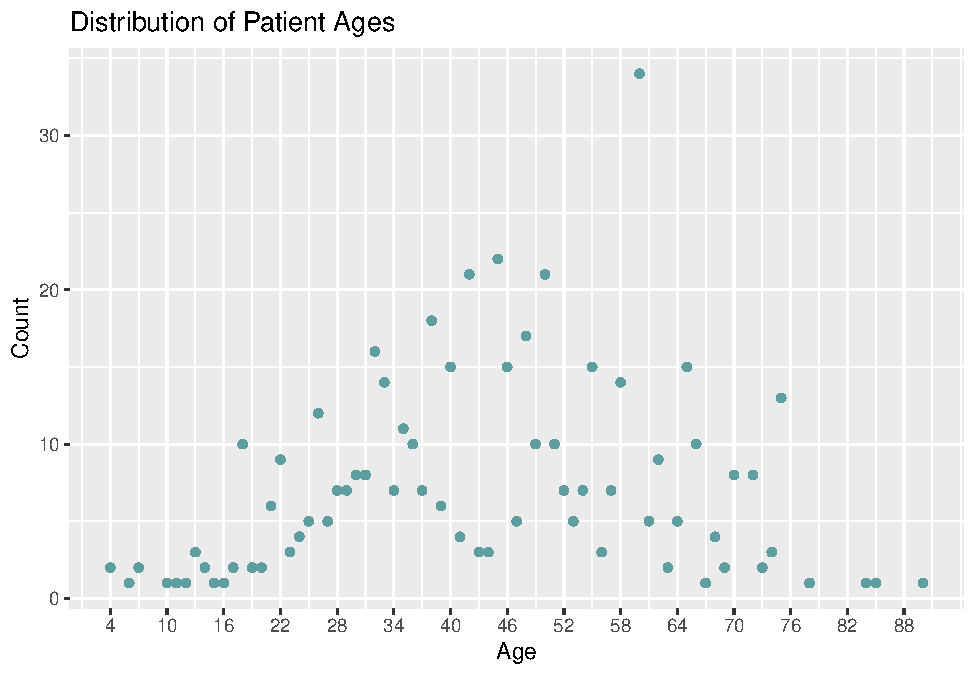
\includegraphics{LiverDisease_files/figure-latex/unnamed-chunk-9-1.pdf}

\textbackslash subsection\{Direct\_Bilirubin\} Again, we can see that
levels of Direct\_Bilirubin are also high for patients with liver
diseases.

\begin{Shaded}
\begin{Highlighting}[]
\CommentTok{# Plotting distributions of Total_Bilirubin versus liver diseases}
\NormalTok{training }\OperatorTok\StringTok{ }
\StringTok{  }\KeywordTok{ggplot}\NormalTok{(}\KeywordTok{aes}\NormalTok{(}\KeywordTok{as.numeric}\NormalTok{(}\KeywordTok{row.names}\NormalTok{(training)),Direct_Bilirubin, }\DataTypeTok{color=}\NormalTok{Disease)) }\OperatorTok{+}
\StringTok{  }\KeywordTok{geom_boxplot}\NormalTok{() }\OperatorTok{+}
\StringTok{  }\KeywordTok{labs}\NormalTok{(}\DataTypeTok{y=}\StringTok{"Direct_Bilirubin"}\NormalTok{, }\DataTypeTok{x =} \StringTok{"Number of patients"}\NormalTok{)}\OperatorTok{+}
\StringTok{  }\KeywordTok{facet_wrap}\NormalTok{( }\OperatorTok{~}\StringTok{ }\NormalTok{Disease) }\OperatorTok{+}
\StringTok{  }\KeywordTok{ggtitle}\NormalTok{(}\StringTok{"Distribution of Direct_Bilirubin w.r.t liver disease"}\NormalTok{)}
\end{Highlighting}
\end{Shaded}

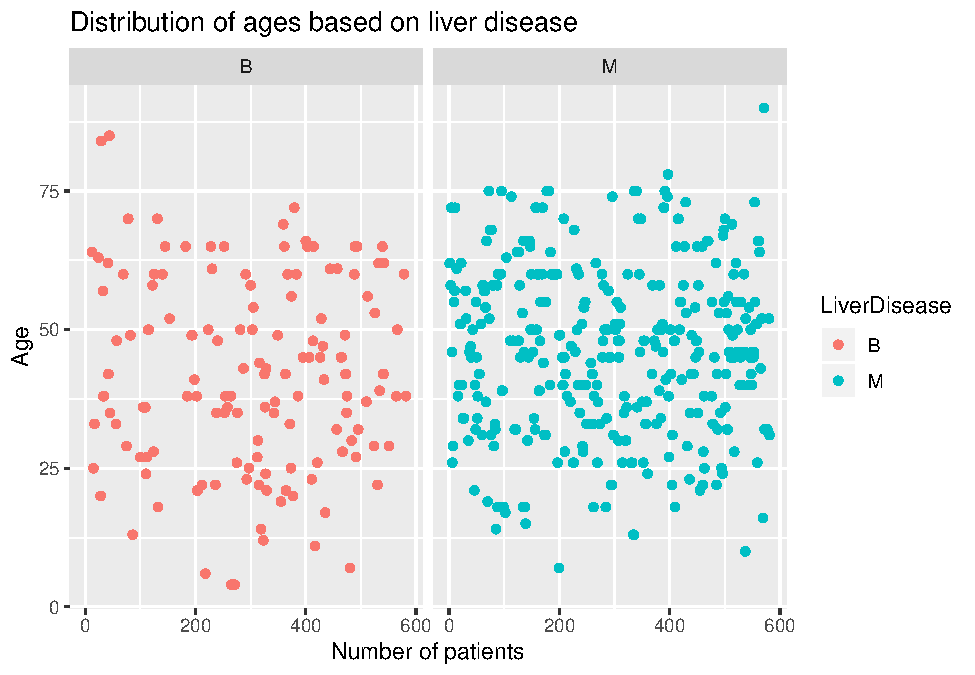
\includegraphics{LiverDisease_files/figure-latex/unnamed-chunk-10-1.pdf}
The correlations indicate that there is a weak correlation between liver
disease and bilirubin. Though, the values are comparatively higher with
liver diseases.

\begin{Shaded}
\begin{Highlighting}[]
\NormalTok{subset_train <-}\StringTok{ }\NormalTok{training[}\KeywordTok{c}\NormalTok{(}\StringTok{"Total_Bilirubin"}\NormalTok{,}\StringTok{"Direct_Bilirubin"}\NormalTok{)]}
\NormalTok{subset_train <-}\StringTok{ }\KeywordTok{transform}\NormalTok{(subset_train, }\DataTypeTok{Disease=} \KeywordTok{ifelse}\NormalTok{(training}\OperatorTok{$}\NormalTok{Disease}\OperatorTok{==}\StringTok{"M"}\NormalTok{, }\DecValTok{1}\NormalTok{,}\DecValTok{0}\NormalTok{))}
\KeywordTok{cor}\NormalTok{(subset_train) }
\end{Highlighting}
\end{Shaded}

\begin{verbatim}
##                  Total_Bilirubin Direct_Bilirubin   Disease
## Total_Bilirubin        1.0000000        0.8584292 0.2065553
## Direct_Bilirubin       0.8584292        1.0000000 0.2347388
## Disease                0.2065553        0.2347388 1.0000000
\end{verbatim}

\subsection{Alkaline Phosphotase}

Alkaline phosphatase (ALP) is an enzyme in a person's blood that helps
break down proteins. We observe that levels of Alkaline Phosphotase are
comparatively high for patients with liver diseases.

\begin{Shaded}
\begin{Highlighting}[]
\CommentTok{# Plotting distributions of Alkaline Phosphotase versus liver diseases}
\NormalTok{training }\OperatorTok\StringTok{ }
\StringTok{  }\KeywordTok{ggplot}\NormalTok{(}\KeywordTok{aes}\NormalTok{(}\KeywordTok{as.numeric}\NormalTok{(}\KeywordTok{row.names}\NormalTok{(training)),Alkaline_Phosphotase, }\DataTypeTok{color=}\NormalTok{Disease)) }\OperatorTok{+}
\StringTok{  }\KeywordTok{geom_boxplot}\NormalTok{() }\OperatorTok{+}
\StringTok{  }\KeywordTok{labs}\NormalTok{(}\DataTypeTok{y=}\StringTok{"Alkaline Phosphotase"}\NormalTok{, }\DataTypeTok{x =} \StringTok{"Number of patients"}\NormalTok{)}\OperatorTok{+}
\StringTok{  }\KeywordTok{facet_wrap}\NormalTok{( }\OperatorTok{~}\StringTok{ }\NormalTok{Disease) }\OperatorTok{+}
\StringTok{  }\KeywordTok{ggtitle}\NormalTok{(}\StringTok{"Distribution of Alkaline Phosphotase w.r.t liver disease"}\NormalTok{)}
\end{Highlighting}
\end{Shaded}

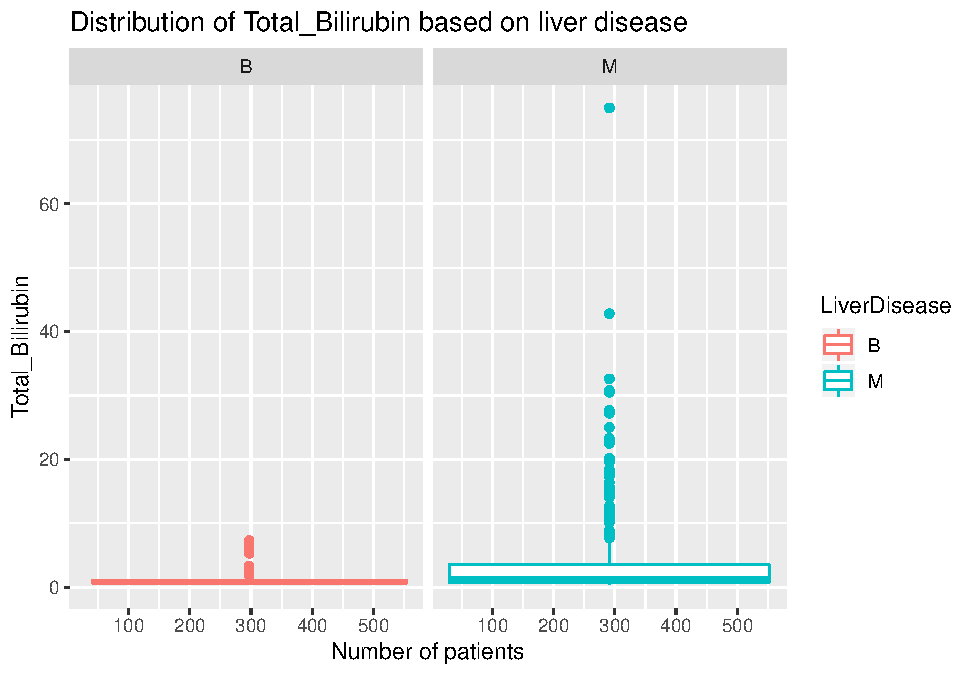
\includegraphics{LiverDisease_files/figure-latex/unnamed-chunk-12-1.pdf}

\textbackslash subsection\{Alamine\_Aminotransferase\} Alanine
aminotransferase (ALT) is an enzyme found primarily in the liver and
kidney. ALT is increased with liver damage and is used to screen liver
disease. We can see that levels of Alamine\_Aminotransferase are high
for patients with liver diseases.

\begin{Shaded}
\begin{Highlighting}[]
\CommentTok{# Plotting distributions of Alamine Aminotransferase versus liver diseases}
\NormalTok{training }\OperatorTok\StringTok{ }
\StringTok{  }\KeywordTok{ggplot}\NormalTok{(}\KeywordTok{aes}\NormalTok{(}\KeywordTok{as.numeric}\NormalTok{(}\KeywordTok{row.names}\NormalTok{(training)),Alamine_Aminotransferase, }\DataTypeTok{color=}\NormalTok{Disease)) }\OperatorTok{+}
\StringTok{  }\KeywordTok{geom_boxplot}\NormalTok{() }\OperatorTok{+}
\StringTok{  }\KeywordTok{labs}\NormalTok{(}\DataTypeTok{y=}\StringTok{"Alamine Aminotransferase"}\NormalTok{, }\DataTypeTok{x =} \StringTok{"Number of patients"}\NormalTok{)}\OperatorTok{+}
\StringTok{  }\KeywordTok{facet_wrap}\NormalTok{( }\OperatorTok{~}\StringTok{ }\NormalTok{Disease) }\OperatorTok{+}
\StringTok{  }\KeywordTok{ggtitle}\NormalTok{(}\StringTok{"Distribution of Alamine Aminotransferase w.r.t liver disease"}\NormalTok{) }
\end{Highlighting}
\end{Shaded}

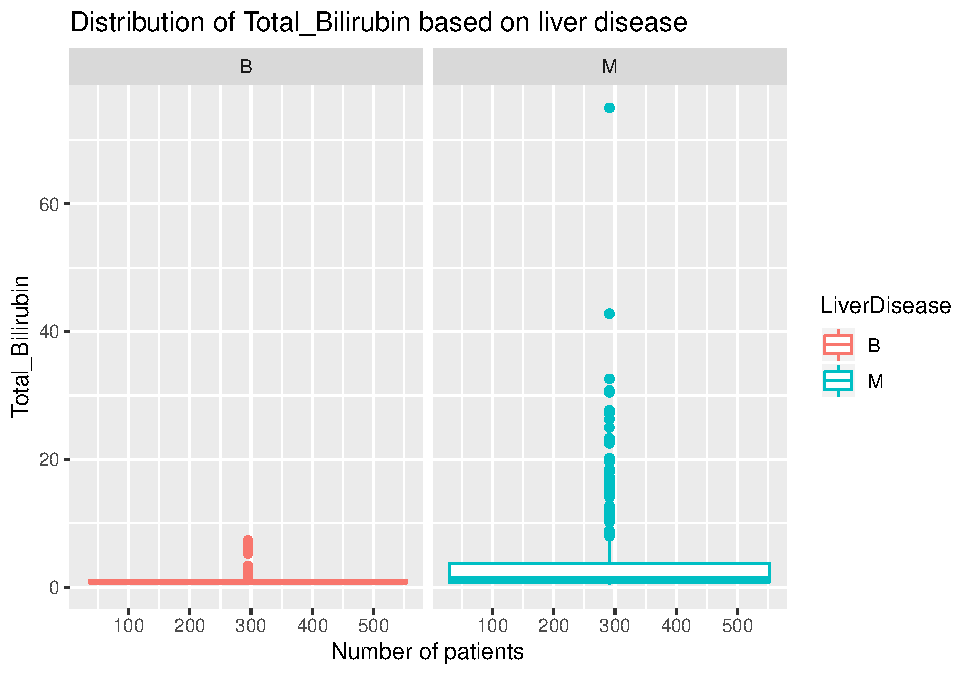
\includegraphics{LiverDisease_files/figure-latex/unnamed-chunk-13-1.pdf}

\textbackslash subsection\{Aspartate\_Aminotransferase\} Aspartate
aminotransferase (AST) is an enzyme found in cells throughout the body
but mostly in the heart and liver. In healthy individuals, levels of AST
in the blood are low. When liver is damaged, they release AST into the
blood thus raising the levels.We can see that levels of AST are
comparatively high for very few patients with liver diseases.

\begin{Shaded}
\begin{Highlighting}[]
\CommentTok{# Plotting distributions of Aspartate_Aminotransferase versus liver diseases}
\NormalTok{training }\OperatorTok\StringTok{ }
\StringTok{  }\KeywordTok{ggplot}\NormalTok{(}\KeywordTok{aes}\NormalTok{(}\KeywordTok{as.numeric}\NormalTok{(}\KeywordTok{row.names}\NormalTok{(training)),Aspartate_Aminotransferase, }\DataTypeTok{color=}\NormalTok{Disease)) }\OperatorTok{+}
\StringTok{  }\KeywordTok{geom_boxplot}\NormalTok{() }\OperatorTok{+}
\StringTok{  }\KeywordTok{labs}\NormalTok{(}\DataTypeTok{y=}\StringTok{"Aspartate Aminotransferase"}\NormalTok{, }\DataTypeTok{x =} \StringTok{"Number of patients"}\NormalTok{)}\OperatorTok{+}
\StringTok{  }\KeywordTok{facet_wrap}\NormalTok{( }\OperatorTok{~}\StringTok{ }\NormalTok{Disease) }\OperatorTok{+}
\StringTok{  }\KeywordTok{ggtitle}\NormalTok{(}\StringTok{"Distribution of Aspartate Aminotransferase w.r.t liver disease"}\NormalTok{) }
\end{Highlighting}
\end{Shaded}

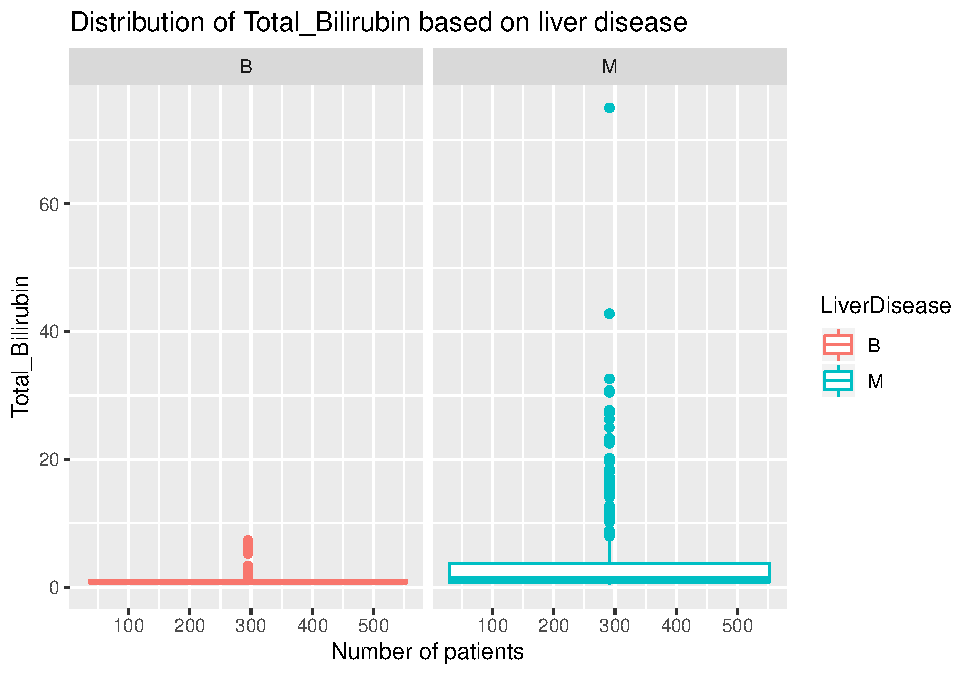
\includegraphics{LiverDisease_files/figure-latex/unnamed-chunk-14-1.pdf}

\subsection{Total Protiens}

The total protein test measures the total amount albumin and globulin in
your body. It is used as part of your routine health checkup. The
anaysis suggest that there is no correlation between liver disease and
total protiens in our dataset. So, we will not use it for model
training.

\begin{Shaded}
\begin{Highlighting}[]
\CommentTok{# Plotting distributions of Total Protiens versus liver diseases}
\NormalTok{training }\OperatorTok\StringTok{ }
\StringTok{  }\KeywordTok{ggplot}\NormalTok{(}\KeywordTok{aes}\NormalTok{(}\KeywordTok{as.numeric}\NormalTok{(}\KeywordTok{row.names}\NormalTok{(training)),Total_Protiens, }\DataTypeTok{color=}\NormalTok{Disease)) }\OperatorTok{+}
\StringTok{  }\KeywordTok{geom_boxplot}\NormalTok{() }\OperatorTok{+}
\StringTok{  }\KeywordTok{labs}\NormalTok{(}\DataTypeTok{y=}\StringTok{"Total Protiens"}\NormalTok{, }\DataTypeTok{x =} \StringTok{"Number of patients"}\NormalTok{)}\OperatorTok{+}
\StringTok{  }\KeywordTok{facet_wrap}\NormalTok{( }\OperatorTok{~}\StringTok{ }\NormalTok{Disease) }\OperatorTok{+}
\StringTok{  }\KeywordTok{ggtitle}\NormalTok{(}\StringTok{"Distribution of Total Protiens w.r.t liver disease"}\NormalTok{) }
\end{Highlighting}
\end{Shaded}

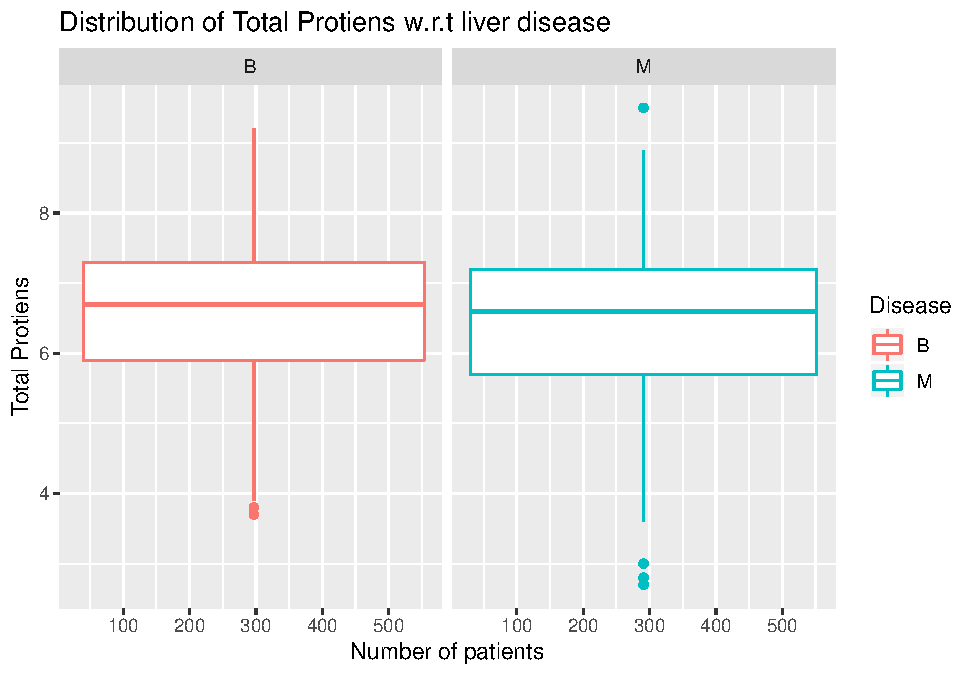
\includegraphics{LiverDisease_files/figure-latex/unnamed-chunk-15-1.pdf}

\subsection{Albumin}

Albumin is a protein made by your liver. Albumin helps keep fluid in
your bloodstream so it doesn't leak into other tissues. Low albumin
levels can indicate a problem with your liver or kidneys. In our
dataset, this variable has no strong correlation with the liver disease.

\begin{Shaded}
\begin{Highlighting}[]
\CommentTok{# Plotting distributions of Albumin versus liver diseases}
\NormalTok{training }\OperatorTok\StringTok{ }
\StringTok{  }\KeywordTok{ggplot}\NormalTok{(}\KeywordTok{aes}\NormalTok{(}\KeywordTok{as.numeric}\NormalTok{(}\KeywordTok{row.names}\NormalTok{(training)),Albumin, }\DataTypeTok{color=}\NormalTok{Disease)) }\OperatorTok{+}
\StringTok{  }\KeywordTok{geom_boxplot}\NormalTok{() }\OperatorTok{+}
\StringTok{  }\KeywordTok{labs}\NormalTok{(}\DataTypeTok{y=}\StringTok{"Albumin"}\NormalTok{, }\DataTypeTok{x =} \StringTok{"Number of patients"}\NormalTok{)}\OperatorTok{+}
\StringTok{  }\KeywordTok{facet_wrap}\NormalTok{( }\OperatorTok{~}\StringTok{ }\NormalTok{Disease) }\OperatorTok{+}
\StringTok{  }\KeywordTok{ggtitle}\NormalTok{(}\StringTok{"Distribution of Albumin w.r.t liver disease"}\NormalTok{) }
\end{Highlighting}
\end{Shaded}

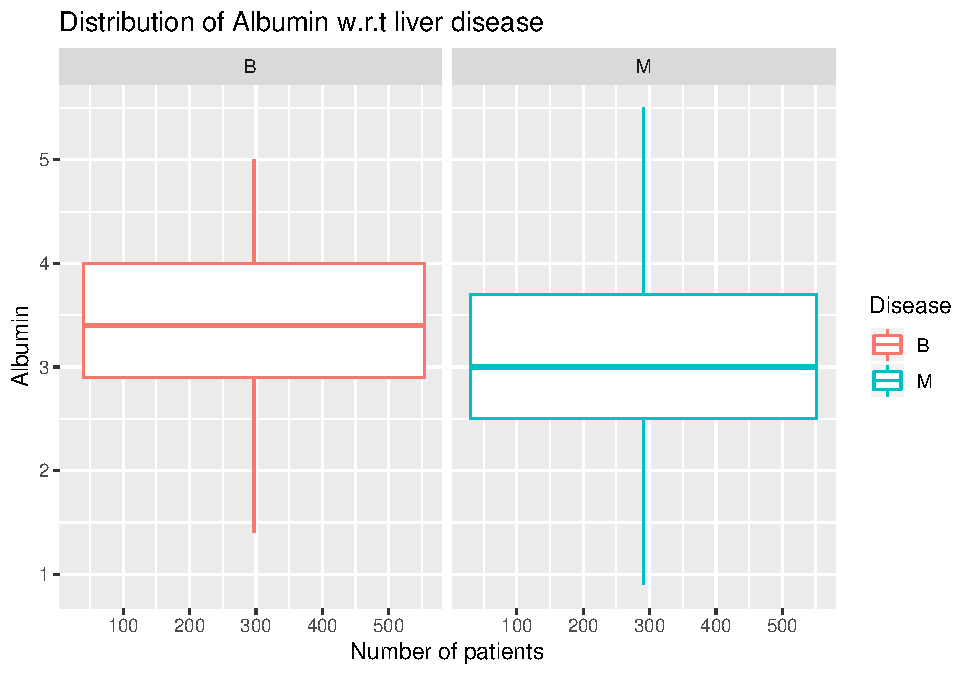
\includegraphics{LiverDisease_files/figure-latex/unnamed-chunk-16-1.pdf}
\textbackslash subsection\{Albumin\_and\_Globulin\_Ratio\} There are two
classes of proteins are found in the blood. They are important for body
growth, development, and health. They form the structural part of most
organs and make up enzymes and hormones that regulate body functions. We
can see that these protiens have no correlation with the liver disease.

\begin{Shaded}
\begin{Highlighting}[]
\CommentTok{# Plotting distributions of Albumin versus liver diseases}
\NormalTok{training }\OperatorTok\StringTok{ }
\StringTok{  }\KeywordTok{ggplot}\NormalTok{(}\KeywordTok{aes}\NormalTok{(}\KeywordTok{as.numeric}\NormalTok{(}\KeywordTok{row.names}\NormalTok{(training)),Albumin_and_Globulin_Ratio, }\DataTypeTok{color=}\NormalTok{Disease)) }\OperatorTok{+}
\StringTok{  }\KeywordTok{geom_boxplot}\NormalTok{() }\OperatorTok{+}
\StringTok{  }\KeywordTok{labs}\NormalTok{(}\DataTypeTok{y=}\StringTok{"Albumin and Globulin Ratio"}\NormalTok{, }\DataTypeTok{x =} \StringTok{"Number of patients"}\NormalTok{)}\OperatorTok{+}
\StringTok{  }\KeywordTok{facet_wrap}\NormalTok{( }\OperatorTok{~}\StringTok{ }\NormalTok{Disease) }\OperatorTok{+}
\StringTok{  }\KeywordTok{ggtitle}\NormalTok{(}\StringTok{"Distribution of Albumin and Globulin Ratio w.r.t liver disease"}\NormalTok{) }
\end{Highlighting}
\end{Shaded}

\begin{verbatim}
## Warning: Removed 4 rows containing non-finite values (stat_boxplot).
\end{verbatim}

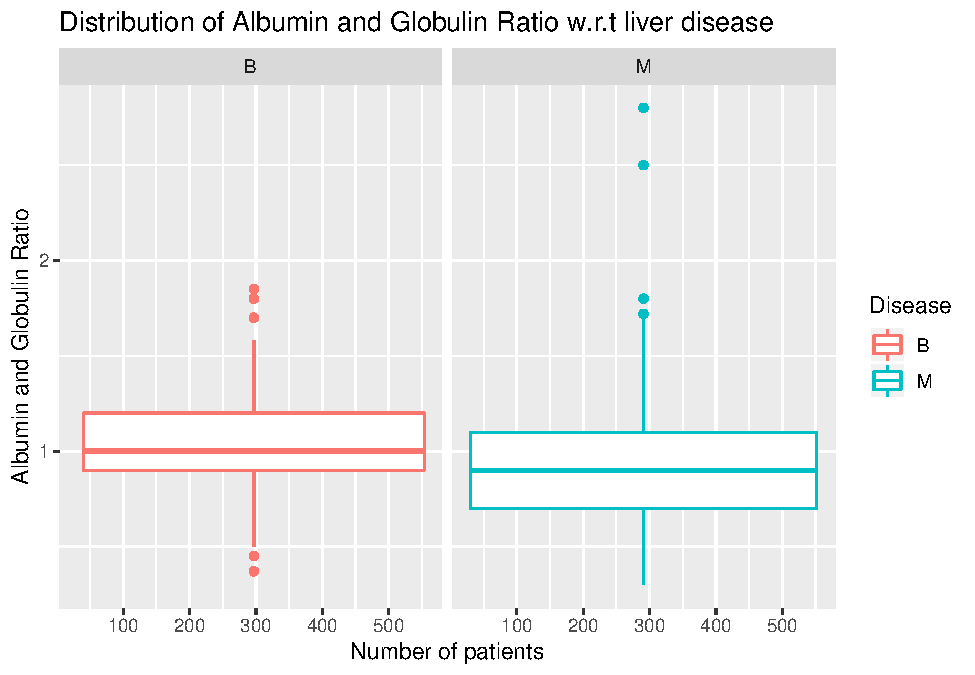
\includegraphics{LiverDisease_files/figure-latex/unnamed-chunk-17-1.pdf}
We can that Bilirubin enzymes are highly correlated with the liver
disease. We are going to use these 5 variables to predict the liver
disease.

\begin{Shaded}
\begin{Highlighting}[]
\NormalTok{samples <-}\StringTok{ }\NormalTok{training }
\NormalTok{samples <-}\StringTok{ }\KeywordTok{transform}\NormalTok{(samples, }\DataTypeTok{Disease=} \KeywordTok{ifelse}\NormalTok{(training}\OperatorTok{$}\NormalTok{Disease}\OperatorTok{==}\StringTok{"M"}\NormalTok{, }\DecValTok{1}\NormalTok{,}\DecValTok{0}\NormalTok{))}
\NormalTok{samples<-}\KeywordTok{within}\NormalTok{(samples, }\KeywordTok{rm}\NormalTok{(Age,Gender,Total_Protiens,Albumin,Albumin_and_Globulin_Ratio))}
\KeywordTok{colnames}\NormalTok{(samples)<-}\KeywordTok{c}\NormalTok{ (}\StringTok{"T_Bil"}\NormalTok{,}\StringTok{"T_Bil"}\NormalTok{,}\StringTok{"A_Phos"}\NormalTok{,}\StringTok{"Al_Amin"}\NormalTok{,}\StringTok{"Asp_Amino"}\NormalTok{,}\StringTok{"Disease"}\NormalTok{)}
\KeywordTok{cor}\NormalTok{(samples)}
\end{Highlighting}
\end{Shaded}

\begin{verbatim}
##               T_Bil     T_Bil    A_Phos   Al_Amin Asp_Amino   Disease
## T_Bil     1.0000000 0.8584292 0.2356568 0.1686019 0.2003604 0.2065553
## T_Bil     0.8584292 1.0000000 0.2681528 0.1897871 0.2219221 0.2347388
## A_Phos    0.2356568 0.2681528 1.0000000 0.1692258 0.2156400 0.1782120
## Al_Amin   0.1686019 0.1897871 0.1692258 1.0000000 0.7317857 0.1616705
## Asp_Amino 0.2003604 0.2219221 0.2156400 0.7317857 1.0000000 0.1488358
## Disease   0.2065553 0.2347388 0.1782120 0.1616705 0.1488358 1.0000000
\end{verbatim}

\begin{thebibliography}{9}
\bibitem{cad} 
Ethan Du-Crowa, Lucy Warrenb, Susan M Astleya and Johan Hullemanc,"Is there a safety-net effect with Computer-Aided Detection (CAD)?", Medical Imaging 2019.
\bibitem{ld}
Eugene, R., Sorrell, Michael F.; Maddrey, Willis C., "Schiff's Diseases of the Liver", 10th Edition, Lippincott Williams \& Wilkins by Schiff.

\bibitem{bendi}
Bendi,  Venkata . R, M. S. Prasad Babu, and N. B. Venkateswarlu, "Critical Comparative Study of Liver Patients from USA and INDIA: An Exploratory Analysis", International Journal of Computer Science Issues, May 2012.


\end{thebibliography}


\end{document}
